\chapter{Pseudorandom functions}\label{4-Pseudorandom-functions}

In the last lecture we saw the notion of \emph{pseudorandom generators},
and introduced the \textbf{PRG conjecture}, which stated that there
exists a pseudorandom generator mapping \(n\) bits to \(n+1\) bits. We
have seen the \emph{length extension} theorem, which states that given
such a pseudorandom generator, there exists a generator mapping \(n\)
bits to \(m\) bits for an arbitrarily large polynomial \(m(n)\). But can
we extend it even further? Say, to \(2^n\) bits? Does this question even
make sense? And why would we want to do that? This is the topic of this
lecture.

At a first look, the notion of extending the output length of a
pseudorandom generator to \(2^n\) bits seems nonsensical. After all, we
want our generator to be \emph{efficient} and just writing down the
output will take exponential time. However, there is a way around this
conundrum. While we can't efficiently write down the full output, we can
require that it would be possible, given an index
\(i\in \{0,\ldots,2^n-1\}\), to compute the \(i^{th}\) bit of the output
in polynomial time.\footnote{In this course we will often index strings
  and numbers starting from zero rather than one, and so typically index
  the coordinates of a string \(y\in \{0,1\}^N\) as \(0,\ldots,N-1\)
  rather than \(1,\ldots,N\). But we will not be religious about it and
  occasionally ``lapse'' into one-based indexing. In almost all cases,
  this makes no difference.} That is, we require that the function
\(i \mapsto G(s)_i\) is efficiently computable and (by security of the
pseudorandom generator) indistinguishable from a function that maps each
index \(i\) to an independent random bit in \(\{0,1\}\). This is the
notion of a \emph{pseudorandom function generator} which is a bit subtle
to define and construct, but turns out to have a great many applications
in cryptography.

\hypertarget{prfdef}{}
\begin{definition}[Pseudorandom Function Generator] \label[definition]{prfdef}

An efficiently computable function \(F\) taking two inputs
\(s\in\{0,1\}^n\) and \(i\in \{0,\ldots,2^n-1\}\) and outputting a
single bit \(F(s,i)\) is a \emph{pseudorandom function (PRF) generator}
if for every polynomial time adversary \(A\) outputting a single bit and
polynomial \(p(n)\), if \(n\) is large enough then:

\begin{equation*}
 \left| \E_{s\in\{0,1\}^n}[ A^{F(s,\cdot)}(1^n)] - \E_{H \leftarrow_R [2^n]\rightarrow\{0,1\}}[A^H(1^n)] \right| < 1/p(n) \;.
\end{equation*}

\end{definition}

Some notes on notation are in order. The input \(1^n\) is simply a
string of \(n\) ones, and it is a typical cryptography convention to
assume that such an input is always given to the adversary. This is
simply because by ``polynomial time adversary'' we really mean
polynomial in \(n\) (which is our key size or security
parameter)\footnote{This also allows us to be consistent with the notion
  of ``polynomial in the size of the input.''}. The notation
\(A^{F(s,\cdot)}\) means that \(A\) has \emph{black box} (also known as
\emph{oracle}) access to the function that maps \(i\) to \(F(s,i)\).
That is, \(A\) can choose an index \(i\), query the box and get
\(F(s,i)\), then choose a new index \(i'\), query the box to get
\(F(s,i')\), and so on for a polynomial number of queries. The notation
\(H \leftarrow_R [2^n] \rightarrow \{0,1\}\) means that \(H\) is a
completely random function that maps every index \(i\) to an independent
and random different bit.

\hypertarget{randfuncs}{}
\begin{remark}[Completely Random Functions] \label[remark]{randfuncs}

This notion of a randomly chosen function can be difficult to wrap your
mind around. Try to imagine a table of all of the strings in
\(\{0, 1\}^n\). We now go to each possible input, randomly generate a
bit to be its output, and write down the result in the table. When we're
done, we have a length \(2^n\) lookup table that maps each input to an
output that was generated uniformly at random and independently of all
other outputs. This lookup table is now our random function \(H\).

In practice it's too cumbersome to actually generate all \(2^n\) bits,
and sometimes in theory it's convenient to think of each output as
generated only after a query is made. This leads to adopting the
\emph{lazy evaluation model}. In the lazy evaluation model, we imagine
that a lazy person is sitting in a room with the same lookup table as
before, but with all entries blank. If someone makes some query
\(H(s)\), the lazy person checks if the entry for \(s\) in the lookup
table is blank. If so, the lazy evaluator generates a random bit, writes
down the result for \(s\), and returns it. Otherwise, if an output has
already been generated for \(s\) previously (because \(s\) has been
queried before), the lazy evaluator simply returns this value. Can you
see why this model is more convenient in some ways?

One last way to think about how a completely random function is
determined is to first observe that there exist a total of \(2^{2^n}\)
functions from \(\{0, 1\}^n\) to \(\{0, 1\}\) (can you see why? It may
be easier to think of them as functions from \([2^n]\) to \(\{0, 1\}\)).
We choose one of them uniformly at random to be \(H\), and it's still
the case that for any given input \(s\) the result \(H(s)\) is \(0\) or
\(1\) with equal probability independent of any other input.

Regardless of which model we use to think about generating \(H\), after
we've chosen \(H\) and put it in a black box, the behavior of \(H\) is
in some sense ``deterministic'' because given the same query it will
always return the same result. However, before we ever make any given
query \(s\) we can only guess \(H(s)\) correctly with probability
\(\tfrac{1}{2}\), because without previously observing \(H(s)\) it is
effectively random and undecided to us (just like in the lazy evaluator
model).

\end{remark}

\begin{pause} \label[pause]{4-Now-would-be-a-fantast}

Now would be a fantastic time to stop and think deeply about the three
constructions in the remark above, and in particular why they are all
equivalent. If you don't feel like thinking then at the very least you
should make a mental note to come back later if you're confused, because
this idea will be very useful down the road.

\end{pause}

Thus, the notation \(A^H\) in the PRF definition means \(A\) has access
to a completely random black box that returns a random bit for any new
query made, and on previously seen queries returns the same bit as
before. Finally one last note: below we will identify the set
\([2^n] = \{0,\ldots,2^n-1\}\) with the set \(\{0,1\}^n\) (there is a
one to one mapping between those sets using the binary representation),
and so we will treat \(i\) interchangeably as a number in \([2^n]\) or a
string in \(\{0,1\}^n\).

Informally, if \(F\) is a pseudorandom function generator, then if we
choose a random string \(s\) and consider the function \(f_s\) defined
by \(f_s(i) = F(s,i)\), no efficient algorithm can distinguish between
black box access to \(f_s(\cdot)\) and black box access to a completely
random function (see \cref{prfmodelfig}). Notably, black box access
implies that a priori the adversary does not know which function it's
querying. From the adversary's point of view, they query some oracle
\(O\) (which behind the scenes is either \(f_s(\cdot)\) or \(H\)), and
must decide if \(O = f_s(\cdot)\) or \(O = H\). Thus often instead of
talking about a pseudorandom function generator we will refer to a
\emph{pseudorandom function collection} \(\{ f_s \}\) where by that we
mean the map \(F(s,i)=f_s(i)\) is a pseudorandom function generator.

\begin{figure}
\centering
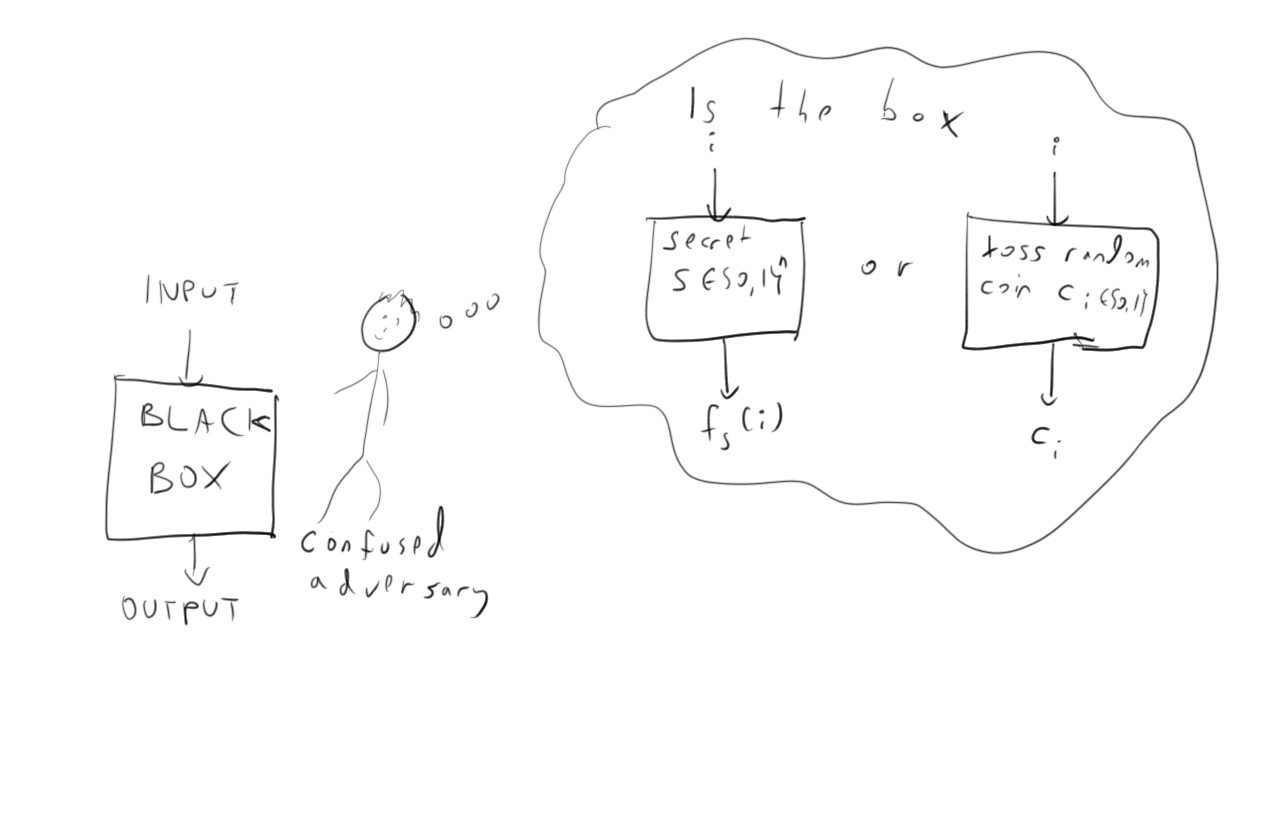
\includegraphics[width=\textwidth, height=0.25\paperheight, keepaspectratio]{../figure/pseudorandom_function.jpg}
\caption{In a pseudorandom function, an adversary cannot tell whether
they are given a black box that computes the function
\(i \mapsto F(s,i)\) for some secret \(s\) that was chosen at random and
fixed, or whether the black box computes a completely random function
that tosses a fresh random coin whenever it's given a new input \(i\).}
\label{prfmodelfig}
\end{figure}

In the next lecture we will see the proof of following theorem (due to
Goldreich, Goldwasser, and Micali)

\hypertarget{prffromprgthmone}{}
\begin{theorem}[PRFs from PRGs] \label[theorem]{prffromprgthmone}

Assuming the PRG conjecture, there exists a secure pseudorandom function
generator.

\end{theorem}

But before we see the proof of \cref{prffromprgthmone}, let us see why
pseudorandom functions could be useful.

\section{One time passwords (e.g.~Google Authenticator, RSA ID,
etc.)}\label{4-One-time-passwords-egG}

Until now we have talked about the task of \emph{encryption}, or
protecting the \emph{secrecy} of messages. But the task of
\emph{authentication}, or protecting the \emph{integrity} of messages is
no less important. For example, consider the case that you receive a
software update for your PC, phone, car, pacemaker, etc. over an open
channel such as an unencrypted Wi-Fi connection. The contents of that
update are not secret, but it is of crucial importance that it was
unchanged from the message sent out by the company and that no malicious
attacker had modified the code. Similarly, when you log into your bank,
you might be much more concerned about the possibility of someone
impersonating you and cleaning out your account than you are about the
secrecy of your information.

Let's start with a very simple scenario which we'll call \textbf{the
login problem}. \textbf{Alice} and \textbf{Bob} share a key as before,
but now Alice wants to simply prove her identity to Bob. What makes this
challenging is that this time they need to contend with not the passive
eavesdropping Eve but the active adversary \textbf{Mallory}, who
completely controls the communication channel between them and can
modify (or \emph{mall}) any message that they send. Specifically for the
identity proving case, we think of the following scenario. Each instance
of such an \textbf{identification protocol} consists of some interaction
between Alice and Bob that ends with Bob deciding whether to accept it
as authentic or reject as an impersonation attempt. Mallory's goal is to
fool Bob into accepting her as Alice.

The most basic way to try to solve the login problem is by simply using
a \emph{password}. That is, if we assume that Alice and Bob can share a
key, we can treat this key as some secret password \(p\) that was
selected at random from \(\{0,1\}^n\) (and hence can only be guessed
with probability \(2^{-n}\)). Why doesn't Alice simply send \(p\) to Bob
to prove to him her identity? A moment's thought shows that this would
be a very bad idea. Since Mallory is controlling the communication line,
she would learn \(p\) after the first identification attempt and could
then easily impersonate Alice in future interactions. However, we seem
to have just the tool to protect the secrecy of \(p\)---
\emph{encryption}. Suppose that Alice and Bob share a secret key \(k\)
and an additional secret password \(p\). Wouldn't a simple way to solve
the login problem be for Alice to send to Bob an encryption of the
password \(p\)? After all, the security of the encryption should
guarantee that Mallory can't learn \(p\), right?

\begin{pause} \label[pause]{4-This-would-be-a-good-t}

This would be a good time to stop reading and try to think for yourself
whether using a secure encryption to encrypt \(p\) would guarantee
security for the login problem. (No really, stop and think about it.)

\end{pause}

The problem is that Mallory does not have to learn the password \(p\) in
order to impersonate Alice. For example, she can simply record the
message Alice \(c_1\) sends to Bob in the first session and then
\emph{replay} it to Bob in the next session. Since the message is a
valid encryption of \(p\), then Bob would accept it from Mallory! (This
is known as a \emph{replay attack} and is a common attack one needs to
protect against in cryptographic protocols.) One can try to put in
countermeasures to defend against this particular attack, but its
existence demonstrates that secrecy of the password does not guarantee
security of the login protocol.

\subsection{How do pseudorandom functions help in the login
problem?}\label{4-How-do-pseudorandom-fu}

The idea is that they create what's known as a \emph{one time password}.
Alice and Bob will share an index \(s\in\{0,1\}^n\) for the pseudorandom
function generator \(\{ f_s \}\). When Alice wants to prove to Bob her
identity, Bob will choose a random \(i\leftarrow_R\{0,1\}^n\), and send
\(i\) to Alice, and then Alice will send
\(f_s(i),f_s(i+1),\ldots,f_s(i+\ell-1)\) to Bob where \(\ell\) is some
parameter (you can think of \(\ell=n\) for simplicity). Bob will check
that indeed \(y=f_s(i)\) and if so accept the session as authentic.

The formal protocol is as follows:

\paragraph{Protocol} \texttt{PRF-Login}\textbf{:}

\begin{itemize}
\tightlist
\item
  Shared input: \(s\in\{0,1\}^n\). Alice and Bob treat it as a seed for
  a pseudorandom function generator \(\{ f_s \}\).
\item
  In every session Alice and Bob do the following:

  \begin{enumerate}
  \def\labelenumi{\arabic{enumi}.}
  \tightlist
  \item
    Bob chooses a random \(i\leftarrow_R[2^n]\) and sends \(i\) to
    Alice.
  \item
    Alice sends \(y_1,\ldots,y_\ell\) to Bob where \(y_j = f_s(i+j-1)\).
  \item
    Bob checks that for every \(j\in\{1,\ldots,\ell\}\),
    \(y_j = f_s(i+j-1)\) and if so accepts the session; otherwise he
    rejects it.
  \end{enumerate}
\end{itemize}

As we will see it's not really crucial that the input \(i\) (which is
known in crypto parlance as a \emph{nonce}) is random. What is crucial
is that it never repeats itself, to foil a replay attack. For this
reason in many applications Alice and Bob compute \(i\) as a function of
the current time (for example, the index of the current minute based on
some agreed-upon starting point), and hence we can make it into a one
message protocol. Also the parameter \(\ell\) is sometimes chosen to be
deliberately short so that it will be easy for people to type the values
\(y_1,\ldots,y_\ell\).

\begin{marginfigure}
\centering
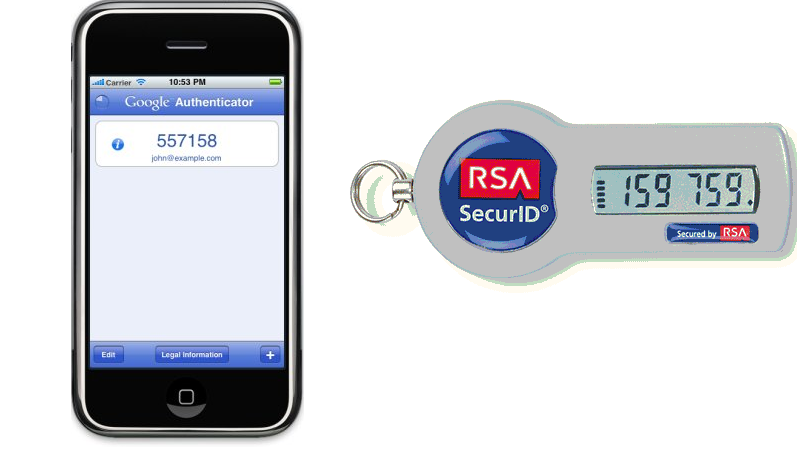
\includegraphics[width=\linewidth, height=1.5in, keepaspectratio]{../figure/google-authenticator.jpg}
\caption{The Google Authenticator app is one popular example of a
one-time password scheme using pseudorandom functions. Another example
is RSA's SecurID token.}
\label{tmplabelfig}
\end{marginfigure}

\emph{Why is this secure?} The key to understanding schemes using
pseudorandom functions is to imagine what would happen if instead of a
\emph{pseudo} random function, \(f_s\) would be an \emph{actual} random
function. In a truly random function, every one of the values
\(f_s(0),\ldots,f_s(2^n-1)\) is chosen independently and uniformly at
random from \(\{0,1\}\). One useful way to imagine this is using the
concept of ``lazy evaluation''. We can think of \(f_S\) as determined by
tossing \(2^n\) different coins for the values \(f(0),\ldots,f(2^n-1)\).
Now consider the case where we don't actually toss the \(i^{th}\) coin
until we need it. The crucial point is that if we have queried the
function in \(T\ll 2^n\) places, then when Bob chooses a random
\(i\in[2^n]\) it is \emph{extremely unlikely} that any one of the set
\(\{i,i+1,\ldots,i+\ell-1\}\) will be one of those locations that we
previously queried. Thus, if the function was truly random, Mallory has
\emph{no information} on the value of the function in these coordinates,
and would be able to predict (or rather, guess) it in all these
locations with probability at most \(2^{-\ell}\).

\begin{pause} \label[pause]{4-Please-make-sure-you-u}

Please make sure you understand the informal reasoning above, since we
will now translate this into a formal theorem and proof.

\end{pause}

\hypertarget{loginprfthm}{}
\begin{theorem}[Login protocol via PRF] \label[theorem]{loginprfthm}

Suppose that \(\{ f_s \}\) is a secure pseudorandom function generator
and Alice and Bob interact using Protocol \texttt{PRF-Login} for some
polynomial number \(T\) of sessions (over a channel controlled by
Mallory). After observing these interactions, Mallory then interacts
with Bob, where Bob follows the protocol's instructions but Mallory has
access to arbitrary efficient computation. Then, the probability that
Bob accepts the interaction is at most \(2^{-\ell}+\mu(n)\) where
\(\mu(\cdot)\) is some negligible function.

\end{theorem}

\begin{proof} \label[proof]{4-This-proof-as-so-many-}

This proof, as so many others in this course, uses an argument via
contradiction. We assume, towards the sake of contradiction, that there
exists an adversary \(M\) (for Mallory) that can break the
identification scheme \texttt{PRF-Login} with probability
\(2^{-\ell}+\epsilon\) after \(T\) interactions. We then construct an
attacker \(A\) that can distinguish access to \(\{ f_s \}\) from access
to a random function in \(poly(T)\) time and with bias at least
\(\epsilon/2\).

How do we construct this adversary \(A\)? The idea is as follows. First,
we prove that if we ran the protocol \texttt{PRF-Login} using an
\emph{actual random} function, then \(M\) would not be able to succeed
in impersonating with probability better than \(2^{-\ell}+negligible\).
Therefore, if \(M\) does do better, then we can use that to distinguish
\(f_s\) from a random function. The adversary \(A\) gets some black box
\(O(\cdot)\) (for \emph{oracle}) and will use it while internally
simulating all the parties--- Alice, Bob and Mallory (using \(M\)) in
the \(T+1\) interactions of the \texttt{PRF-Login} protocol. Whenever
any of the parties needs to evaluate \(f_s(i)\), \(A\) will forward
\(i\) to its black box \(O(\cdot)\) and return the value \(O(i)\). It
will then output \(1\) if an only if \(M\) succeeds in impersonation in
this internal simulation. The argument above showed that if \(O(\cdot)\)
is a truly random function, then the probability that \(A\) outputs
\(1\) is at most \(2^{-\ell}+negligible\) (and so in particular less
than \(2^{-\ell}+\epsilon/2\)). On the other hand, if \(O(\cdot)\) is
the function \(i \mapsto f_s(i)\) for some fixed and random \(s\), then
this probability is at least \(2^{-\ell}+\epsilon\). Thus \(A\) will
distinguish between the two cases with bias at least \(\epsilon/2\). We
now turn to the formal proof:

\textbf{Claim 1:} Let \texttt{PRF-Login*} be the hypothetical variant of
the protocol \texttt{PRF-Login} where Alice and Bob share a completely
random function \(H:[2^n]\rightarrow\{0,1\}\). Then, no matter what
Mallory does, the probability she can impersonate Alice after observing
\(T\) interactions is at most \(2^{-\ell}+(8\ell T)/2^n\).

(If \texttt{PRF-Login*} is easier to prove secure than
\texttt{PRF-Login}, you might wonder why we bother with
\texttt{PRF-Login} in the first place and not simply use
\texttt{PRF-Login*}. The reason is that specifying a random function
\(H\) requires specifying \(2^n\) bits, and so that would be a
\emph{huge} shared key. So \texttt{PRF-Login*} is not a protocol we can
actually run but rather a hypothetical ``mental experiment'' that helps
us in arguing about the security of \texttt{PRF-Login}.)

\textbf{Proof of Claim 1:} Let \(i_1,\ldots,i_{2T}\) be the nonces
chosen by Bob and recieved by Alice in the first \(T\) iterations. That
is, \(i_1\) is the nonce chosen by Bob in the first iteration while
\(i_2\) is the nonce that Alice received in the first iteration (if
Mallory doesn't modify it then \(i_1=i_2\)). Similarly, \(i_3\) is the
nonce chosen by Bob in the second iteration while \(i_4\) is the nonce
received by Alice and so on and so forth. Let \(i\) be the nonce chosen
in the \(T+1^{st}\) iteration in which Mallory tries to impersonate
Alice. We claim that the probability that there exists some
\(j\in\{1,\ldots,2T\}\) such that \(|i-i_j|<2\ell\) is at most
\(8\ell T/2^n\). Indeed, let \(S\) be the union of all the intervals of
the form \(\{ i_j-2\ell+1,\ldots, i_j+2\ell-1 \}\) for
\(1 \leq j \leq 2T\). Since it's a union of \(2T\) intervals each of
length less than \(4\ell\), \(S\) contains at most \(8T\ell\) elements,
so the probability that \(i\in S\) is \(|S|/2^n \leq (8T\ell)/2^n\).
Now, if there does \emph{not} exists a \(j\) such that \(|i-i_j|<2\ell\)
then it means in particular that all the queries to \(H(\cdot)\) made by
either Alice or Bob during the first \(T\) iterations are disjoint from
the interval \(\{ i,i+1,\ldots,i+\ell-1 \}\). Since \(H(\cdot)\) is a
completely random function, the values \(H(i),\ldots,H(i+\ell-1)\) are
chosen uniformly and independently from all the rest of the values of
this function. Since Mallory's message \(y\) to Bob in the \(T+1^{st}\)
iteration depends only on what she observed in the past, the values
\(H(i),\ldots,H(i+\ell-1)\) are \emph{independent} from \(y\), and hence
under this condition that there is no overlap between this interval and
prior queries, the probability that they equal \(y\) is \(2^{-\ell}\).
QED (Claim 1).

The proof of Claim 1 is not hard but it is somewhat subtle, so it's good
to go over it again and make sure you understand it.

Now that we have Claim 1, the proof of the theorem follows as outlined
above. We build an adversary \(A\) to the pseudorandom function
generator from \(M\) by having \(A\) simulate ``inside its belly'' all
the parties Alice, Bob and Mallory and output \(1\) if Mallory succeeds
in impersonating. Since we assumed \(\epsilon\) is non-negligible and
\(T\) is polynomial, we can assume that \((8\ell T)/2^n < \epsilon/2\)
and hence by Claim 1, if the black box is a random function, then we are
in the \texttt{PRF-Login*} setting and Mallory's success will be at most
\(2^{-\ell}+\epsilon/2\). If the black box is \(f_s(\cdot)\), then we
get exactly the \texttt{PRF-Login} setting and hence under our
assumption the success will be at least \(2^{-\ell}+\epsilon\). We
conclude that the difference in probability of \(A\) outputting \(1\)
between the random and pseudorandom case is at least \(\epsilon/2\) thus
contradicting the security of the pseudorandom function generator.

\end{proof}

\hypertarget{outputincprfrem}{}
\begin{remark}[Increasing output length of PRFs] \label[remark]{outputincprfrem}

In the course of constructing this one-time-password scheme from a PRF,
we have actually proven a general statement that is useful on its own:
that we can transform standard PRF which is a collection \(\{ f_s \}\)
of functions mapping \(\{0,1\}^n\) to \(\{0,1\}\), into a PRF where the
functions have a longer output \(\ell\) (see the problem set for a
formal statement of this result) Thus from now on whenever we are given
a PRF, we will allow ourselves to assume that it has any output size
that is convenient for us.

\end{remark}

\section{Message Authentication Codes}\label{4-Message-Authentication}

One time passwords are a tool allowing you to prove your \emph{identity}
to, say, your email server. But even after you did so, how can the
server trust that future communication comes from you and not from some
attacker that can interfere with the communication channel between you
and the server (so called ``man in the middle'' attack)? Similarly, one
time passwords may allow a software company to prove their identity
before they send you a software update, but how do you know that an
attacker does not change some bits of this software update on route
between their servers and your device?

This is where \emph{Message Authentication Codes (MACs)} come into play-
their role is to authenticate not only the \emph{identity} of the
parties but also their \emph{communication}. Once again we have
\textbf{Alice} and \textbf{Bob}, and the adversary \textbf{Mallory} who
can actively modify messages (in contrast to the passive eavesdropper
Eve). Similar to the case to encryption, Alice has a \emph{message}
\(m\) she wants to send to Bob, but now we are not concerned with
Mallory \emph{learning} the contents of the message. Rather, we want to
make sure that Bob gets precisely the message \(m\) sent by Alice.
Actually this is too much to ask for, since Mallory can always decide to
block all communication, but we can ask that either Bob gets precisely
\(m\) or he detects failure and accepts no message at all. Since we are
in the \emph{private key} setting, we assume that Alice and Bob share a
key \(k\) that is unknown to Mallory.

What kind of security would we want? We clearly want Mallory not to be
able to cause Bob to accept a message \(m'\neq m\). But, like in the
encryption setting, we want more than that. We would like Alice and Bob
to be able to use the same key for \emph{many} messages. So, Mallory
might observe the interactions of Alice and Bob on messages
\(m_1,\ldots,m_T\) before trying to cause Bob to accept a message
\(m'_{T+1} \neq m_{T+1}\). In fact, to make our notion of security more
robust, we will even allow Mallory to \emph{choose} the messages
\(m_1,\ldots,m_T\) (this is known as a \emph{chosen message} or
\emph{chosen plaintext} attack). The resulting formal definition is
below:

\hypertarget{MACdef}{}
\begin{definition}[Message Authentication Codes (MAC)] \label[definition]{MACdef}

Let \((S,V)\) (for \emph{sign} and \emph{verify}) be a pair of
efficiently computable algorithms where \(S\) takes as input a key \(k\)
and a message \(m\), and produces a tag \(\tau \in \{0,1\}^*\), while
\(V\) takes as input a key \(k\), a message \(m\), and a tag \(\tau\),
and produces a bit \(b\in\{0,1\}\). We say that \((S,V)\) is a
\emph{Message Authentication Code (MAC)} if:

\begin{itemize}
\tightlist
\item
  For every key \(k\) and message \(m\), \(V_k(m,S_k(m))=1\).\\
\item
  For every polynomial-time adversary \(A\) and polynomial \(p(n)\), it
  is with less than \(1/p(n)\) probability over the choice of
  \(k\leftarrow_R\{0,1\}^n\) that \(A^{S_k(\cdot)}(1^n)=(m',\tau')\)
  such that \(m'\) is \emph{not} one of the messages \(A\) queries and
  \(V_k(m',\tau')=1\).\footnote{Clearly if the adversary outputs a pair
    \((m,\tau)\) that it did query from its oracle then that pair will
    pass verification. This suggests the possibility of a \emph{replay}
    attack whereby Mallory resends to Bob a message that Alice sent him
    in the past. As above, once can thwart this by insisting the every
    message \(m\) begins with a fresh nonce or a value derived from the
    current time.}
\end{itemize}

\end{definition}

If Alice and Bob share the key \(k\), then to send a message \(m\) to
Bob, Alice will simply send over the pair \((m,\tau)\) where
\(\tau = S_k(m)\). If Bob receives a message \((m',\tau')\), then he
will accept \(m'\) if and only if \(V_k(m',\tau')=1\). Mallory now
observes \(t\) rounds of communication of the form \((m_i,S_k(m_i))\)
for messages \(m_1,\ldots,m_t\) of her choice, and her goal is to try to
create a new message \(m'\) that was \emph{not} sent by Alice, but for
which she can forge a valid tag \(\tau'\) that will pass verification.
Our notion of security guarantees that she'll only be able to do so with
negligible probability, in which case the MAC is
\textbf{CMA-secure}.\footnote{A priori you might ask if we should not
  also give Mallory an oracle to \(V_k(\cdot)\) as well. After all, in
  the course of those many interactions, Mallory could also send Bob
  many messages \((m',\tau')\) of her choice, and observe from his
  behavior whether or not these passed verification. It is a good
  exercise to show that adding such an oracle does not change the power
  of the definition, though we note that this is decidedly \emph{not}
  the case in the analogous question for encryption.}

\hypertarget{choosemessages}{}
\begin{remark}[Why can Mallory choose the messages?] \label[remark]{choosemessages}

The notion of a ``chosen message attack'' might seem a little ``over the
top''. After all, Alice is going to send to Bob the messages of
\emph{her} choice, rather than those chosen by her adversary Mallory.
However, as cryptographers have learned time and again the hard way, it
is better to be conservative in our security definitions and think of an
attacker that has as much power as possible. First of all, we want a
message authentication code that will work for \emph{any} sequence of
messages, and so it's better to consider this ``worst case'' setting of
allowing Mallory to choose them. Second, in many realistic settings an
adversary could have some effect on the messages that are being sent by
the parties. This has occurred time and again in cases ranging from web
servers to German submarines in World War II, and we'll return to this
point when we talk about \emph{chosen plaintext} and \emph{chosen
ciphertext} attacks on encryption schemes.

\end{remark}

\hypertarget{strongunforgability}{}
\begin{remark}[Strong unforgability] \label[remark]{strongunforgability}

Some texts (such as Boneh Shoup) define a stronger notion of
unforgability where the adversary cannot even produce new signatures for
messages it \emph{has} queried in the attack. That is, the adversary
cannot produce a valid message-signature pair that it has not seen
before. This stronger definition can be useful for some applications. It
is fairly easy to transform MACs satisfying \cref{MACdef} into MACs
satisfying strong unforgability. In particular, if the signing function
is deterministic, and we use a \emph{canonical verifier algorithm} where
\(V_k(m,\sigma)=1\) iff \(S_k(m)=\sigma\) then weak unforgability
automatically implies strong unforgability since every message has a
single signature that would pass verification (can you see why?).

\end{remark}

\section{MACs from PRFs}\label{4-MACs-from-PRFs}

We now show how pseudorandom function generators yield message
authentication codes. In fact, the construction is so immediate that
much of the more applied cryptographic literature does not distinguish
between these two concepts, and uses the name ``Message Authentication
Codes'' to refer to both MAC's and PRF's. However, since this is not
applied cryptographic literature, the distinction is rather important.

\hypertarget{MACfromPRFthm}{}
\begin{theorem}[MAC Theorem] \label[theorem]{MACfromPRFthm}

Under the PRF Conjecture, there exists a secure MAC.

\end{theorem}

\begin{proof} \label[proof]{4-Let-Fcdotcdot-be-a-sec}

Let \(F(\cdot,\cdot)\) be a secure pseudorandom function generator with
\(n/2\) bits output (as mentioned in \cref{outputincprfrem}, such PRF's
can be constructed from one bit output PRF's). We define
\(S_k(m) = F(k,m)\) and \(V_k(m,\tau)\) to output \(1\) iff
\(F_k(m)=\tau\). Suppose towards the sake of contradiction that there
exists an adversary \(A\) breaks the security of this construction of a
MAC. That is, \(A\) queries \(S_k(\cdot)\) \(poly(n)\) many times and
with probability \(1/p(n)\) for some polynomial \(p\) outputs
\((m',\tau')\) that she did \emph{not} ask for such that
\(F(k,m')=\tau'\).

\end{proof}

We use \(A\) to construct an adversary \(A'\) that can distinguish
between oracle access to a PRF and a random function by simulating the
MAC security game inside \(A'\). Every time \(A\) requests the signature
of some message \(m\), \(A'\) returns \(O(m)\). When \(A\) returns
\((m', \tau')\) at the end of the \(\ensuremath{\mathit{MAC}}\) game,
\(A'\) returns \(1\) if \(O(m') = \tau'\), and \(0\) otherwise. If
\(O(\cdot) = H(\cdot)\) for some completely random function
\(H(\cdot)\), then the value \(H(m')\) would be completely random in
\(\{0,1\}^{n/2}\) and independent of all prior queries. Hence the
probability that this value would equal \(\tau'\) is at most
\(2^{-n/2}\). If instead \(O(\cdot) = F_k(\cdot)\), then by the fact
that \(A\) wins the MAC security game with probability \(1/p(n)\), the
adversary \(A'\) will output \(1\) with probability \(1/p(n)\). That
means that such an adversary \(A'\) can distinguish between an oracle to
\(F_k(\cdot)\) and an oracle to a random function \(H\), which gives us
a contradiction.

\section{Input length extension for MACs and
PRFs}\label{4-Input-length-extension}

So far we required the message to be signed \(m\) to be no longer than
the key \(k\) (i.e., both \(n\) bits long). However, it is not hard to
see that this requirement is not really needed. If our message is
longer, we can divide it into blocks \(m_1,\ldots,m_t\) and sign each
message \((i,m_i)\) individually. The disadvantage here is that the size
of the tag (i.e., MAC output) will grow with the size of the message.
However, even this is not really needed. Because the tag has length
\(n/2\) for length \(n\) messages, we can sign the \emph{tags}
\(\tau_1,\ldots,\tau_t\) and only output those. The verifier can repeat
this computation to verify this. We can continue this way and so get
tags of \(O(n)\) length for arbitrarily long messages. Hence in the
future, whenever we need to, we will assume that our PRFs and MACs can
get inputs in \(\{0,1\}^*\) --- i.e., arbitrarily length strings.

We note that this issue of length extension is actually quite a thorny
and important one in practice. The above approach is not the most
efficient way to achieve this, and there are several more practical
variants in the literature (see Boneh-Shoup Sections 6.4-6.8). Also, one
needs to be very careful on the exact way one chops the message into
blocks and pads it to an integer multiple of the block size. Several
attacks have been mounted on schemes that performed this incorrectly.

\section{Aside: natural proofs}\label{4-Aside-natural-proofs}

Pseudorandom functions play an important role in computational
complexity, where they have been used as a way to give ``barrier
results'' for proving results such as
\(\mathbf{P}\neq \mathbf{NP}\).\footnote{This discussion has more to do
  with computational complexity than cryptography, and so can be safely
  skipped without harming understanding of future material in this
  course.} Specifically, the \href{https://goo.gl/fiH3Pe}{Natural
Proofs} barrier for proving circuit lower bounds says that if strong
enough pseudorandom functions exist, then certain types of arguments are
bound to fail. These are arguments which come up with a property
\(\ensuremath{\mathit{EASY}}\) of a Boolean function
\(f:\{0,1\}^n \rightarrow \{0,1\}\) such that:

\begin{itemize}
\item
  If \(f\) can be computed by a polynomial sized circuit, then it has
  the property \(\ensuremath{\mathit{EASY}}\).
\item
  The property \(\ensuremath{\mathit{EASY}}\) fails to hold for a random
  function with high probability.
\item
  Checking whether \(\ensuremath{\mathit{EASY}}\) holds can be done in
  time polynomial \emph{in the truth table size of \(f\)}. That is, in
  \(2^{O(n)}\) time.
\end{itemize}

A priori these technical conditions might not seem very ``natural'' but
it turns out that many approaches for proving circuit lower bounds (for
restricted families of circuits) have this form. The idea is that such
approaches find a ``non generic'' property of easily computable
function, such as finding some interesting correlations between the some
input bits and the output. These are correlations that are unlikely to
occur in random functions. The lower bound typically follows by
exhibiting a function \(f_0\) that does not have this property, and then
using that to derive that \(f_0\) cannot be efficiently computed by this
particular restricted family of circuits.

The existence of strong enough pseudorandom functions can be shown to
contradict the existence of such a property
\(\ensuremath{\mathit{EASY}}\), since a pseudorandom function can be
computed by a polynomial sized circuit, but it cannot be distinguished
from a random function. While a priori a pseudorandom function is only
secure for polynomial time distinguishers, under certain assumptions it
might be possible to create a pseudorandom function with a seed of size,
say, \(n^5\), that would be secure with respect to adversaries running
in time \(2^{O(n^2)}\).
